\section{Generative Surface Models}
\label{genmodelsec}

In this section we introduce a generative model for meshes  
approximating surfaces with Euler Characteristic $1$. 

State-of-the-art generative models for images, 
such as Generative Adversarial Networks \cite{dcgan}, Pixel autoregressive 
networks \cite{pixelrnn} or Variational Autoencoders \cite{vae}, exploit the locality 
and stationarity of natural images in their probabilistic models,
in the sense that the model satisfies 
\begin{equation}
\label{gen_stab}
p_\theta(x) \approx p_\theta( x_\tau)
\end{equation}
by construction, where $x_\tau$ is a small deformation of a given input $x$. 
This property is obtained via encoders and decoders (or discriminators and generators in the case of GANs) 
with a deep convolutional structure.  

In our setting, we intend to exploit similar geometric stability priors 
on $p(\M)$, a density over the space of meshes that we wish to fit to the data. 
A convenient way to proceed is to use the surface neural network representations 
described in the previous section, and exploit their stability properties to deformations (see Section \ref{stabsection}). 

%explain the disentanglement between 2d mesh and depth
A mesh generative model contains two distinct sources of randomness: 
on the one hand, the randomness associated to the underlying continuous surface, 
which corresponds to shape variability; on the other hand, 
the randomness associated to the discretization of the surface. Whereas 
the former contains the essential semantic meaning, the latter is not 
informative, and to some extent independent of the shape identity. 

In order to formalize this factorization property, we focus initially 
on meshes that can be represented as a depth map over an (irregular) 
2D mesh, referred as \emph{height-field} meshes in the literature.
That is, a mesh $\M=(V, E, F)$ is expressed as 
$(\tilde{\M}, f(\tilde{\M})$, where $\tilde{\M}=(\tilde{V}, \tilde{E}, \tilde{F})$ is now a 2D mesh 
and 
$$f~:~\tilde{V} \to \R$$ 
is a \emph{depth}-map encoding the original node locations $V$, as shown in Figure \ref{genfigure}.

\begin{figure}
\centering
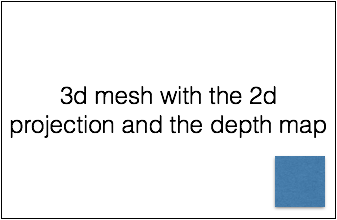
\includegraphics[width=0.7\textwidth]{figures/generative_fig.png}
\label{genfigure}
\caption{A 3D mesh $\M$ is expressed in terms of a ``sampling" 2D irregular mesh $\tilde{\M}$ and a depth scalar field $f$ over $\tilde{\M}$.}  
\end{figure}

In this work, we consider the variational autoencoder framework \cite{vae, vae2}. 
It considers a mixture model of the form 
\begin{equation}
\label{ban1}
p(\M) = \int p_\theta(\M ~|~h) p_0(h) dh~,
\end{equation}
where $h \in \R^S$ is a vector of latent variables. 
As observed by some authors \cite{ganvsvae}, 
mixture models such as (\ref{ban1}) when modeling natural images
suffer to recover high-frequency information. A possible 
explanation for that comes from the fact that variability due to 
geometric deformations is highly nonlinear in the pixel space, 
and is therefore hard to describe with additive mixtures using
unimodal likelihood terms $p_\theta( x ~|~h)$ \cite{superresjoan}. 
However, in surfaces, as described in Section \ref{stabsection}, 
geometric deformations are additive perturbations on the node 
coordinates, making mixture models an appealing choice.

%Variational Autoencoder framework. 
%We describe here the encoder and the decoder model. 
We thus consider a variational auto-encoder associated to model (\ref{ban1}), 
which optimizes the variational lower bound of the data log-likelihood:
\begin{equation}
\min_{\theta, \psi} \frac{1}{L} \sum_{l \leq L} - \E_{ h \sim q_\psi(h ~|~\M_l)} \log p_\theta( \M_l ~|~h) + D_{KL}( q_\psi( h~|~\M_l) ~||~p_0(h) )~.
\end{equation}
We thus need to specify a conditional generative model $p_\theta(\M ~|~h)$, 
a prior distribution $p_0(h)$ and a variational approximation to the posterior
$q_\psi( h ~|~ \M)$, where $\theta$ and $\psi$ denote respectively generative 
and variational trainable parameters.
Based on the height-field representation, we choose for simplicity a separable model of the form
$$p_\theta(\M ~|~h) =  p_\theta( f~|~h, \tilde{\M}) \cdot p(\tilde{\M}) ~,$$
where $\tilde{\M} \sim p(\tilde{\M})$ is a homogenous Poisson point process, 
and $f \sim p_\theta( f~|~h, \tilde{\M})$ is a Normal distribution with 
mean and isotropic covariance parameters given by a surface neural network:
$$p_\theta( f~|~h, \tilde{\M}) = {\cal N}( \mu(h, \tilde{\M}), \sigma^2(h, \tilde{\M}) {\bf 1})~,~\text{with } [ \mu(h, \tilde{\M}), \sigma^2(h, \tilde{\M})] = \Phi_D(\tilde{M}; h)~.$$
The generation step thus proceeds as follows.
we first sample a 2D mesh $\tilde{\M}$ independent of the latent variable $h$, 
and then sample a depth field over $\tilde{\M}$ conditioned on $h$ from the output
of a decoder network $\Phi_D(\tilde{M}; h)$.

Finally, the variational family $q_\psi$ is also a Normal distribution whose parameters 
are obtained from an encoder Surface Neural Network whose last layer is a global pooling that removes 
the spatial localization:
$$q_\psi( h~|~\M) = {\cal N}(\bar{\mu}, \bar{\sigma}^2 {\bf 1})~,~\text{ with }~ [\bar{\mu}, \bar{\sigma}] = \bar{\Phi}_D(\M)~.$$

Comment on the limitations.

Generalization to other Euler Characteristic is immediate. 


